\section*{Этап 1}

\addcontentsline{toc}{section}{Этап 1}

\subsection*{Описание предметной области}

Существует вселенная, где герои живут уже тысячи лет. Новые герои поставляются корпорацией и имеют разный запас здоровья.\\

Есть пользователи, те инопланетные существа, которые покупают героев и зарабатывают на боях своих героев.\\

Герои деруться песнями, с каждым героем корпорация поставляет в комплекте несколько песен, которые постепенно открываются с растущим опытом героя. Песня может измельчаться на ноты, своеобразные "патроны", которые наносят урон.

\addcontentsline{toc}{subsection}{Описание предметной области}

\subsection*{Описание бизнес процессов}

\addcontentsline{toc}{subsection}{Описание бизнес процессов}

При первом входе в игру дается 1000 золота и 0 опыта.\\
    
Игроки покупают героев. У игроков есть валюта, чтобы платить за героев, у героев есть цена.\\

После покупки героев, игроки могут выставлять по одному герою на поле битвы. Участие может принимать несколько игроков и ходят по очереди, тот кто ходит первый определяется рандомом.\\

Перед сражением игрок может выбрать эффект, с которым будет ходить его герой всю битву и песню, которую будет в этой битве исполнять. \\

Герои дерутся между собой песнями. Песни имеют минимальный уровень опыта, который должен иметь герой, чтобы начать их использовать. То есть песни разблокируются постепенно.\\
    
После того, как разыгралось сражение и есть выигравший герой. У всех игроков отнимается 100 золота перераспределяется в пропорциях равных, кол-ву нанесённого урона. \\

Если деньги заканчиваются, игроку необходимо либо купить игровые деньги за валюту, либо открыть лутбокс, который выдаётся каждому игроку раз в день. \\

Есть список пользователей в онлайне, пользователь приглашает другого пользователя в драку и тот либо отклоняет либо принимает заявку на битву.


\subsection*{Сущности}

\addcontentsline{toc}{subsection}{Сущности}

\begin{itemize}
\item \textbf{Стержневые сущности}
\begin{enumerate}
    \item Песня(id, имя, порог\_опыта, id\_героя, урон)
    \item Игрок(id, имя, баланс, статус\_онлайна, хэш\_пароля)
    \item Персонаж(id, имя, цена, стоимость, здоровье, путь\_к\_аватарке)
    \item Эффект(id, название, цена, выносливость, сила, удача, конституция)
    \item Драка(id, время\_начала, id\_локации)
\end{enumerate}

\item \textbf{Ассоциативные сущности}
\begin{enumerate}
    \item Ходы\_в\_драке(номер\_хода, id\_драки, id\_атакующего, id\_атакуемого, урон)
    \item Сделка(id\_игрока, плата)
    \item Сделка\_по\_герою(id\_сделки, id\_героя)
    \item Сделка\_по\_эффекту(id\_сделки, id\_эффекта)
    \item Участник\_драки(id, id\_драки, id\_эффекта\_в\_драке, id\_используемой\_песни, id\_героя, полученный\_опыт, полученное\_золото, позиция)
    \item Герой(id, опыт, id\_персонажа, id\_игрока)
\end{enumerate}

\item \textbf{Характеристические сущности}
\begin{enumerate}
    \item Локация(id, название)
\end{enumerate}
\end{itemize}

\section*{Этап 2}

\addcontentsline{toc}{section}{Этап 2}

\subsection*{Нарисовать ER-диаграмму предметной области}

\addcontentsline{toc}{subsection}{Нарисовать ER-диаграмму предметной области}

\begin{figure}[H]
	\begin{center}
		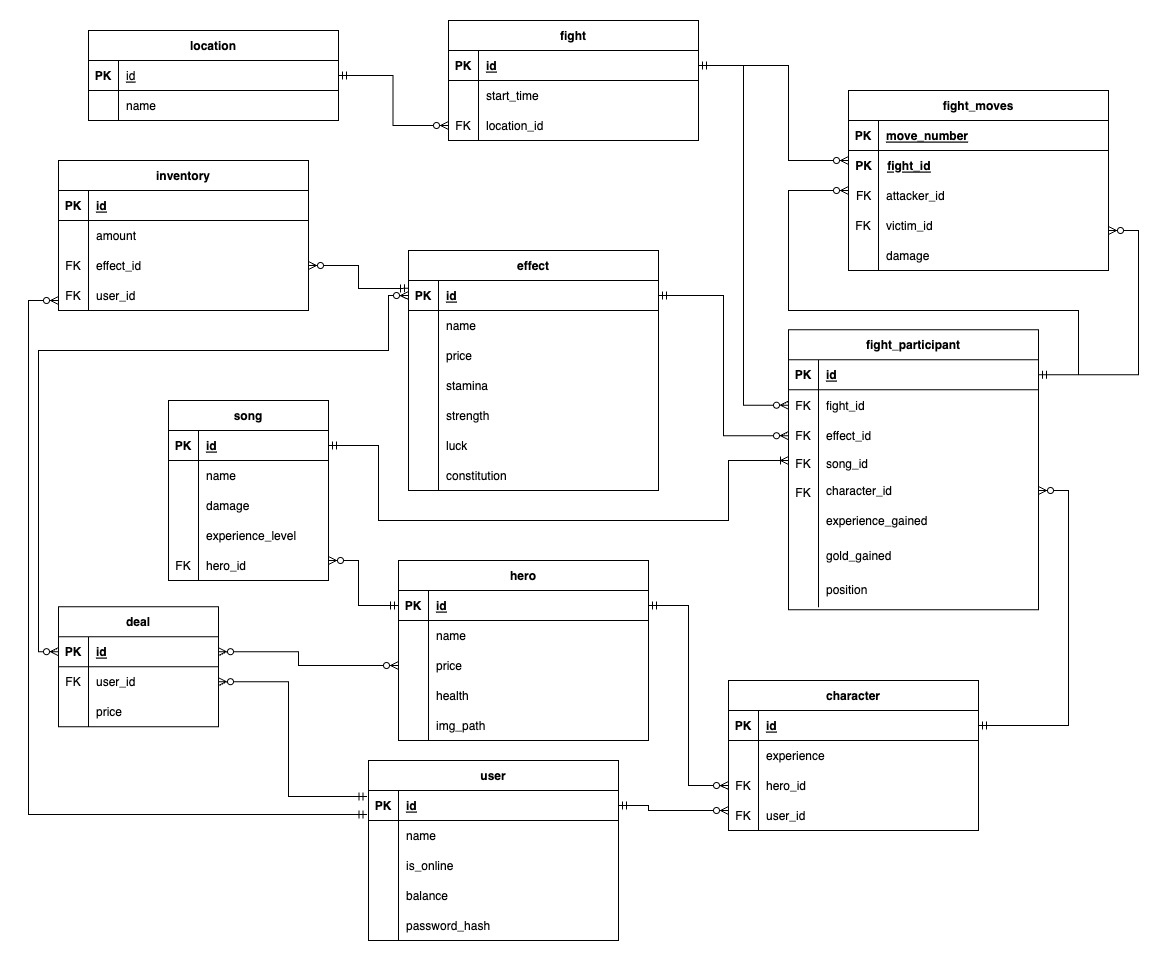
\includegraphics[scale=0.46]{images/ER.jpg}
		\caption{ER-диаграмма предметной области}
	\end{center}
\end{figure}

\subsection*{На основе ER-модели построить даталогическую модель}

\addcontentsline{toc}{subsection}{На основе ER-модели построить даталогическую модель}

\begin{figure}[H]
	\begin{center}
		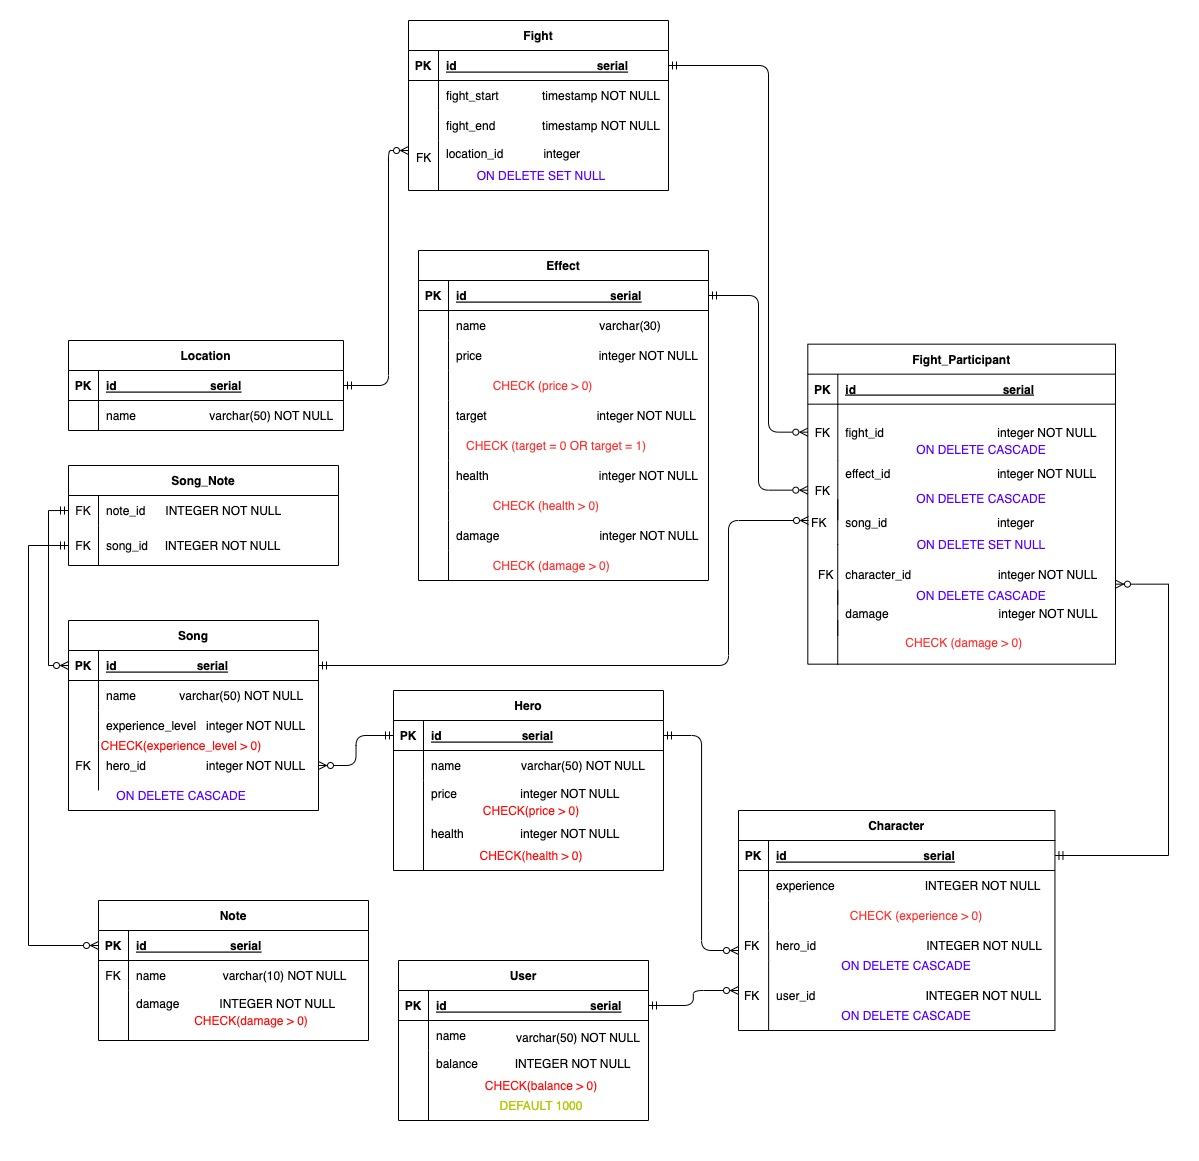
\includegraphics[scale=0.44]{images/Datalogical.jpg}
		\caption{Даталогическая модель}
		\label{pic:pic_name} % название для ссылок внутри кода
	\end{center}
\end{figure}

\newpage

\section*{Этап 3}

\addcontentsline{toc}{section}{Этап 3}

% =======

\subsection*{Создать необходимые объекты базы данных}

\addcontentsline{toc}{subsection}{Создать необходимые объекты базы данных}

% =======

\subsection*{Заполнить созданные таблицы тестовыми данными}

\addcontentsline{toc}{subsection}{Заполнить созданные таблицы тестовыми данными}

% =======

\subsection*{Обеспечить целостность данных при помощи средств языка DDL}

\addcontentsline{toc}{subsection}{Обеспечить целостность данных при помощи средств языка DDL}

% =======

\subsection*{Добавить в базу данных триггеры для обеспечения комплексных ограничений
целостности}

\addcontentsline{toc}{subsection}{Добавить в базу данных триггеры для обеспечения комплексных ограничений
целостности}

\begin{enumerate}
    \item pay\_for\_hero\_log 
    - Тригер для фиксации транзакции игрока за героя(снимает деньги с баланса и добавляет нового героя)

    \item pay\_for\_effect\_log
    - Тригер для фиксации транзакции игрока за эффект(снимает деньги с баланса и добавляет эффект в распоряжение)
\end{enumerate}

% =====

\subsection*{Реализовать функции и процедуры на основе описания бизнес-процессов}

\addcontentsline{toc}{subsection}{Реализовать функции и процедуры на основе описания бизнес-процессов}

\begin{enumerate}
    \item get\_effect\_shop\_info(user\_id) 
    - Возвращает все эффекты, которые можно использовать текущему игроку

    \item buy\_effect(user\_id, effect\_id)
    - Функция покупки эффекта(eсли у пользователя хватает денег на эффект, то покупаем эффект вычитая стоимость из баланса и занося в inventory)

    \item buy\_hero(user\_id, hero\_id)
    - Функция покупки персонажа(если у игрока хватает денег, то вычитаем стоимость персонажа из баланса и добавляем героя связывая с игроком)

    \item get\_base\_character\_info(character\_id, song\_id)
    - Возвращает основную информацию по герою(id, id игрока, id\_в\_драке, здоровье, урон, выносливость, удача)

    \item get\_shop\_info\_for\_user(user\_id)
    - Возвращает список доступных для покупки персонажей с их характеристиками(id, имя, цена, здоровье, аватарка, id\_игрока)

    \item get\_characters\_info\_with\_songs(character\_id[], song\_id[])
    - Возвращает список информаций по участникам драки основываясь участниках и их песнях

    \item get\_upgrade\_character\_info(participant\_info, effect\_id)
    - Изменяет характеристики участника драки в соответствии с выбранным эффектом

    \item get\_available\_effects\_for\_user(user\_id)
    - Выводит список доступных эффектов для выбора для игрока

    \item get\_available\_songs\_for\_character(character\_id)
    - Выводит список доступных песен для героя

    \item begin\_fight(character\_id[], effect\_id[], song\_id[], location\_id)
    - Функция для начала сражения(прогоняет весь матч и возвращает таблицу ходов)

\end{enumerate}

% =====

\subsection*{Произвести анализ использования созданной базы данных}

\addcontentsline{toc}{subsection}{Произвести анализ использования созданной базы данных}

\subsubsection*{Выявить наиболее часто используемые запросы к объектам базы данных}

\addcontentsline{toc}{subsubsection}{Выявить наиболее часто используемые запросы к объектам базы данных}

\subsubsection*{Результаты представить в виде текстового описания}

\addcontentsline{toc}{subsubsection}{Результаты представить в виде текстового описания}

\subsection*{Создать индексы и доказать, что они полезны для вашей базы данных}

\addcontentsline{toc}{subsection}{Создать индексы и доказать, что они полезны для вашей базы данных}

\subsubsection*{Доказательство должно быть приведено в виде текстового описания}

\addcontentsline{toc}{subsubsection}{Доказательство должно быть приведено в виде текстового описания}
